\section{Soft Particles and Biomedical Implications}\label{sec:soft}

When the oscillating particle itself possesses a permeable shell, momentum transport across the particle boundary couples
directly with the response of the porous substrate, modifying both the magnitude of the wall-induced resistance and the
frequency windows of positive added mass. To isolate the role of particle structure, we fix a glycocalyx-like substrate
($\alpha_p=20$, $\beta_p=0$, $\varepsilon=1$) and examine how the shell permeability $\alpha_s$, the core ratio $\kappa$,
and the interfacial parameters reshape the near-wall dynamics, before assessing the implications for acoustofluidic cell
sorting and the physical boundaries of the model.

\subsection{Shell permeability and core size}\label{sec:soft_results}

\begin{figure*}[t]
  \centering
  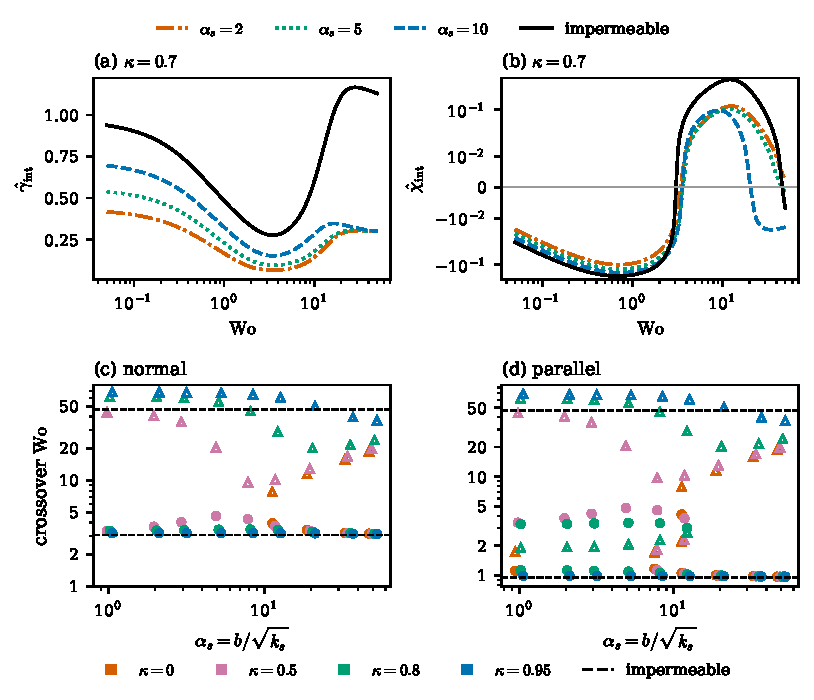
\includegraphics[width=\linewidth]{figures/fig6_soft.pdf}
  \caption{Soft core--shell particles near a glycocalyx-like layer ($\alpha_p=20$, $\beta_p=0$, $\varepsilon=1$).
  (a,b) Damping $\hat\gamma_{\rm int}$ and reactive coefficient $\hat\chi_{\rm int}$ against $\Wo$ for $\kappa=0.7$ and
  $\alpha_s=2,5,10$, compared with an impermeable sphere (normal oscillation). (c,d) All crossover Womersley numbers
  against $\alpha_s$ for $\kappa=0,0.5,0.8,0.95$ (circles: upward; triangles: downward); dashed: impermeable sphere.
  (c) Normal, (d) parallel oscillation.}
  \label{fig:soft}
\end{figure*}

Introducing a permeable shell suppresses the wall-induced damping roughly as the square of the particle's own unbounded
drag. As shown in \cref{fig:soft}(a) for $\kappa=0.7$, the steady wall-induced damping drops from $0.94$ for an
impermeable sphere to $0.70$, $0.54$, and $0.42$ for $\alpha_s=10$, $5$, and $2$, while the finite-frequency minimum near
$\Wo\approx3.5$ falls from $0.28$ to $0.07$. \finding{This quadratic suppression follows directly from the leading
reflection of the Neumann series in \cref{sec:closure}: both the dipole scattered by the particle and the force it
experiences in the reflected flow scale with its unbounded drag ratio $\Omega=F_\infty/F_\infty^{\rm rigid}$, where
$F_\infty^{\rm rigid}$ is the unbounded force on an impermeable sphere of equal outer radius, so that $\gamma_{\rm int}$
scales approximately as $\Omega^2$. Denoting the rigid-sphere wall-induced damping by $\gamma_{\rm int}^{\rm rigid}$, the
computed steady ratio $\gamma_{\rm int}/\gamma_{\rm int}^{\rm rigid}$ equals $0.58$, $0.74$, and $0.87$ for $\alpha_s=5$,
$10$, and $20$ ($\kappa=0.7$), closely tracking $\Omega^2=0.64$, $0.79$, and $0.89$, where $\Omega$ itself reflects the
Debye--Bueche--Brinkman drag reduction caused by flow through the
shell~\cite{brinkman1949calculation,ollila2012hydrodynamic}.} The reactive coefficient in \cref{fig:soft}(b) retains its
lower crossover near $\Wo\approx3$--$4$, whereas its positive maximum decreases by roughly a factor of four. Mapping all
crossovers against $\alpha_s$ in \cref{fig:soft}(c,d) reveals that the crossover structure depends non-monotonically on
particle architecture and can vanish altogether. Thin shells ($\kappa=0.95$) behave essentially as impermeable spheres,
with $\Wo_c^{\uparrow}\approx3.18$ (normal) and $0.99$ (parallel) across all $\alpha_s$. By contrast, homogeneous porous
spheres ($\kappa=0$) exhibit no crossover in normal oscillation for $\alpha_s\le8$, leaving their wall-induced added mass
negative at every frequency; for larger $\alpha_s$, the positive window reappears, with $\Wo_c^{\uparrow}=3.94$ at
$\alpha_s=12$ decreasing towards the impermeable limit. Intermediate cores produce the richest behaviour: for
$\kappa=0.5$, the normal crossover varies non-monotonically with $\alpha_s$, peaking at $4.6$ for $\alpha_s=5$, while in
parallel oscillation the low crossover near $\Wo\approx1$ disappears for $\alpha_s\le5$ and the first crossover jumps to
$\Wo=3.4$--$4.8$. For $\kappa=0.8$ and $\alpha_s\le12$, parallel oscillation exhibits two separate positive windows,
arising from the same potential--vortical separation mechanism identified in \cref{sec:woc}, whereby a permeable
particle---like a permeable layer---weakens and delays the potential image relative to the vortical contribution. The
upper downward crossover also drops substantially, from $46$ for the impermeable sphere to $8$--$20$ for $\kappa=0$ and for
$\kappa=0.5$ with $\alpha_s\ge8$, demonstrating that the crossover spectrum encodes information about both the particle
and the substrate.

\begin{table}[t]
\caption{Sensitivity to the slip length and the shell stress jump (normal oscillation, $\varepsilon=1$, $\alpha_p=20$,
$\beta_p=0$). For the impermeable sphere, $\hat\ell_c$ is the slip length on $r=b$; for the soft particle
($\kappa=0.7$, $\alpha_s=5$) it is the core slip length.}
\label{tab:sensitivity}
\begin{ruledtabular}
\begin{tabular}{lcccc}
Case & $\hat\gamma_{\rm int}(\Wo\to0)$ & $\hat\gamma_{\rm int}(\Wo=3)$ & $\hat\chi_{\rm int}(\Wo=3)$ & $\Wo_c^{\uparrow}$\\
\hline
Impermeable, $\hat\ell_c=0$ & $0.937$ & $0.281$ & $-0.0051$ & $3.06$\\
Impermeable, $\hat\ell_c=0.25$ & $0.639$ & $0.152$ & $+0.0018$ & $2.97$\\
Impermeable, $\hat\ell_c=0.5$ & $0.544$ & $0.125$ & $+0.0104$ & $2.82$\\
Soft, $\hat\ell_c=0$, $\beta_s=0$ & $0.539$ & $0.097$ & $-0.0228$ & $3.66$\\
Soft, $\hat\ell_c=0.5$ & $0.495$ & $0.080$ & $-0.0240$ & $3.86$\\
Soft, $\beta_s=-0.5$ & $0.629$ & $0.125$ & $-0.0318$ & $3.84$\\
Soft, $\beta_s=0.5$ & $0.374$ & $0.062$ & $-0.0058$ & $3.20$\\
\end{tabular}
\end{ruledtabular}
\end{table}

The relative importance of the two interfacial parameters held fixed in \cref{fig:soft} depends strongly on whether the
particle is impermeable or soft, as quantified in \cref{tab:sensitivity}. On an impermeable sphere, a surface slip length
$\hat\ell_c=0.5$ reduces the steady wall-induced damping by $42\%$ and lowers $\Wo_c^{\uparrow}$ from $3.06$ to $2.82$. On
the inner core of a soft particle ($\kappa=0.7$, $\alpha_s=5$), however, the same slip length alters the damping by only
$8\%$, because most of the relative flow passes through the permeable shell rather than shearing along the core.
Conversely, the shell stress-jump coefficient exerts a pronounced influence: varying $\beta_s$ across $\pm0.5$ shifts the
steady damping by $-31\%$ and $+17\%$ and moves $\Wo_c^{\uparrow}$ between $3.20$ and $3.84$. A positive $\beta_s$, like a
positive $\beta_p$, eases tangential momentum exchange across the porous boundary and weakens the wall interaction. Taken
together, \cref{fig:soft} and \cref{tab:sensitivity} show that a permeable shell can lower near-wall damping by up to a
factor of four and eliminate the positive-added-mass window entirely, suggesting that soft, polyethylene glycol
(PEG)-like shells substantially reduce the hydrodynamic resistance experienced by drug-delivery carriers driven near mucus
layers~\cite{pangeni2023airway}, although the present model does not describe penetration into the mucus itself.

\subsection{Acoustofluidic contrast between cell-like particles}\label{sec:acoustic_results}

\begin{figure*}[t]
  \centering
  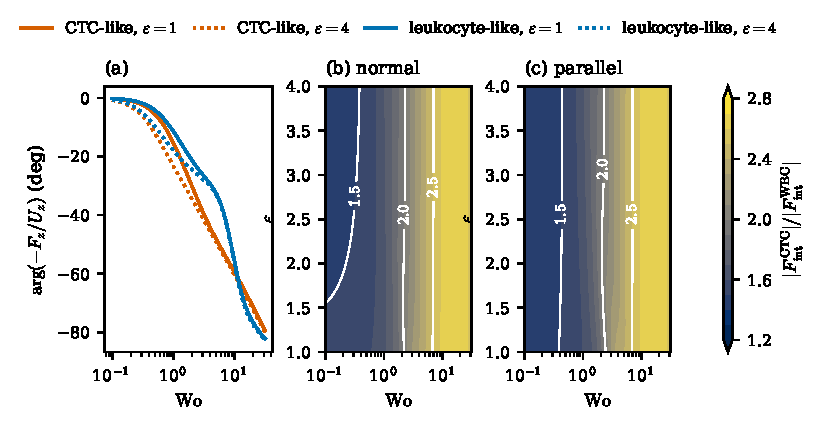
\includegraphics[width=\linewidth]{figures/fig7_acoustic.pdf}
  \caption{Circulating tumour cell (CTC)-like ($\kappa=0.9$, $\alpha_s=20$) and leukocyte-like (white blood cell, WBC;
  $\kappa=0.7$, $\alpha_s=5$) particles of equal outer radius near an endothelial-like layer ($\alpha_p=20$, $\beta_p=0$).
  (a) Phase $\arg(-F_z/U_z)$ of the total normal resistance
  against $\Wo$ at $\varepsilon=1$ and $4$ (normal). (b,c) Ratio $|F^{\rm CTC}_{\rm int}|/|F^{\rm WBC}_{\rm int}|$ of the
  wall-induced force magnitudes in the $(\Wo,\varepsilon)$ plane; white contours mark $1.5$, $2$ and $2.5$. (b) Normal, (c)
  parallel oscillation.}
  \label{fig:acoustic}
\end{figure*}

To illustrate the implications for acoustofluidic sorting~\cite{wu2019acoustofluidic,hossein2023review},
\cref{fig:acoustic} compares a stiffer circulating tumour cell (CTC)-like particle ($\kappa=0.9$, $\alpha_s=20$) with a
softer leukocyte-like (white blood cell, WBC) particle ($\kappa=0.7$, $\alpha_s=5$) of identical outer radius near an
endothelial-like layer ($\alpha_p=20$, $\beta_p=0$). The chosen parameters (\cref{tab:params}) are representative rather
than fitted to specific cell lines. As shown in \cref{fig:acoustic}(a), the phase $\arg(-F_z/U_z)$ of the total normal
resistance differs between the two particles by up to $13^\circ$ near $\Wo\approx3$, whereas the contrast falls below
$1^\circ$ for $\Wo\lesssim0.3$. Across the $(\Wo,\varepsilon)$ plane in \cref{fig:acoustic}(b,c), the wall-induced force
magnitude $|F^{\rm CTC}_{\rm int}|$ of the CTC-like particle is $1.4$ to $2.7$ times larger than $|F^{\rm WBC}_{\rm int}|$
for the leukocyte-like particle. At $\Wo=0.1$, this ratio lies between $1.45$ and $1.53$, closely matching the value
$1.40$ predicted by the $\Omega^2$ scaling from their respective steady drag ratios of $0.95$ and $0.80$, and it depends
primarily on $\Wo$ and only weakly on $\varepsilon$. Nevertheless, the wall interaction constitutes a large fraction of the
total force only close to the substrate and at low to moderate frequency: at $\varepsilon=1$, $|F_{\rm int}|/|F_\infty|$
equals $0.78$ (normal) at $\Wo=0.1$ but drops to $0.04$ at $\Wo=10$, so that at high $\Wo$ most of the force contrast
originates from the unbounded resistance itself. Consequently, near-wall hydrodynamic sorting by softness is most
effective at $\Wo=O(1)$, where both the phase contrast and the wall-induced force remain appreciable; predicting
quantitative trajectory separation in a specific channel will require coupling these resistance spectra to a
device-specific acoustic radiation-force model.

Finally, the physical scope of the present formulation should be borne in mind when applying these results. As
established in \cref{sec:validation}, the dipolar closure is accurate to $5\%$ in normal oscillation and $1.5\%$ in
parallel oscillation at $\varepsilon=1$, and to better than $1\%$ for $\varepsilon\ge2$, while the independent
finite-element benchmark at $\varepsilon=1$ confirms that both the force magnitudes and the crossover frequencies
$\Wo_c$, $\Wo_c^{\uparrow}$, and $\Wo_c^{\downarrow}$ are faithfully captured. Because the closure neglects multipoles of
order $l\ge2$, it does not resolve near-contact lubrication, so the regime $\varepsilon<1$---relevant to probes pressed
directly into a surface brush---requires a higher-order multipole or direct numerical treatment. The model also assumes
rigid porous matrices, a substrate thickness exceeding both $\sqrt{k_p\mu_p/\mu}$ and $h$, pure translation without
rotation (\cref{sec:geometry}), and Brinkman viscosity ratios equal to unity. Moreover, because positive stress-jump
coefficients act as interfacial energy sources (\cref{app:checks}), the physically admissible range is restricted to
$\beta_s,\beta_p\le0.5$ for the configurations studied here. Relaxing the rigid-matrix and semi-infinite assumptions to
include poroelastic deformation of the glycocalyx~\cite{batalha2026elasto} or finite substrate thickness is expected to
modify primarily the high-frequency branch, where the oscillating flow penetrates deeply into the porous layer.
